\chapter{More numeric results on reinforcement learning}
\label{appendix:reinforcement_learning}

\begin{figure}[H]
    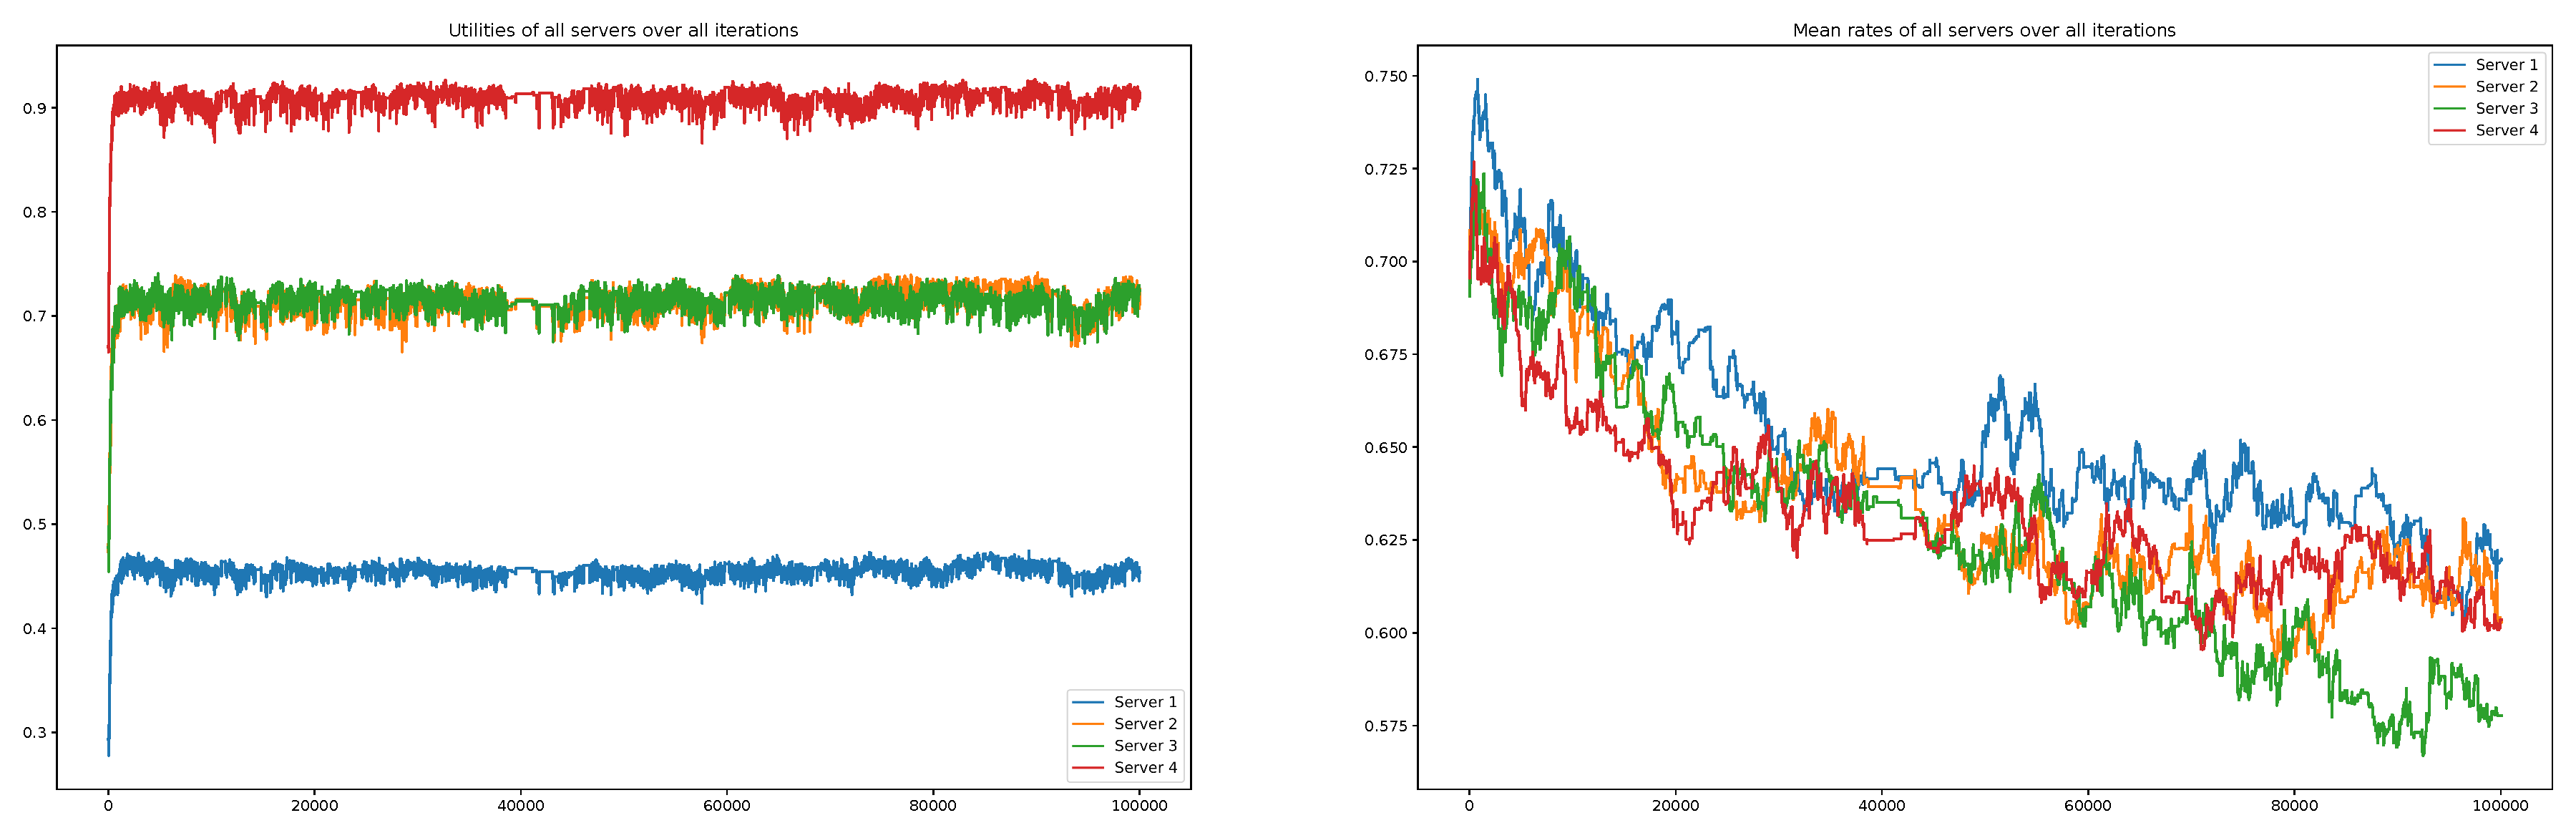
\includegraphics[width=\textwidth]{chapters/00_appendix/03_more_rl_results/Bin/utility_3_eps/u3_1_e0.eps}
    \caption{Utilities and mean service rate of servers from the reinforcement
    learning run using utility function \(U_k^{(3)}\) with \(e = 0\) and
    \(100000\) time steps}
    \label{fig:RL_utility3_1_e0}
\end{figure}

\begin{figure}[H]
    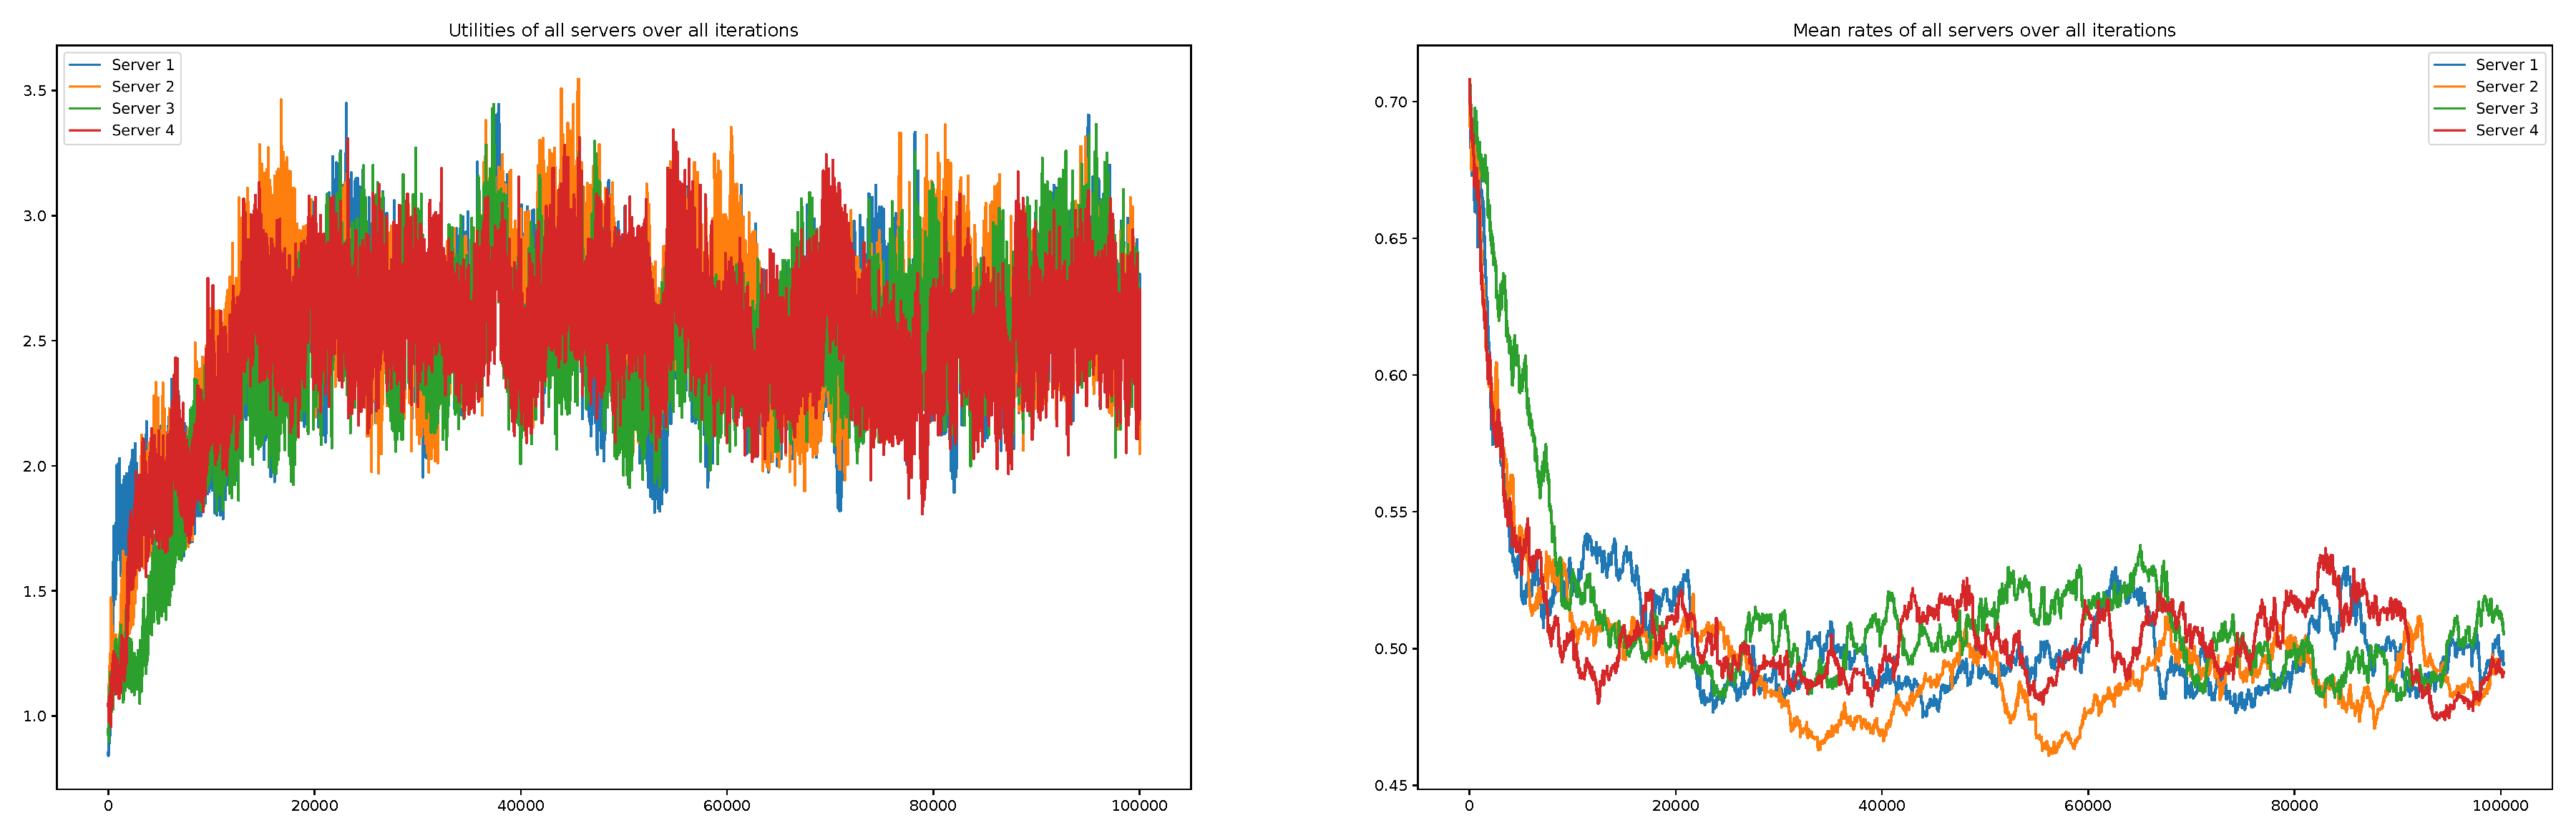
\includegraphics[width=\textwidth]{chapters/00_appendix/03_more_rl_results/Bin/utility_3_eps/u3_1_e05.eps}
    \caption{Utilities and mean service rate of servers from the reinforcement
    learning run using utility function \(U_k^{(3)}\) with \(e = 0.5\) and
    \(100000\) time steps}
    \label{fig:RL_utility3_1_e05}
\end{figure}

\begin{figure}[H]
    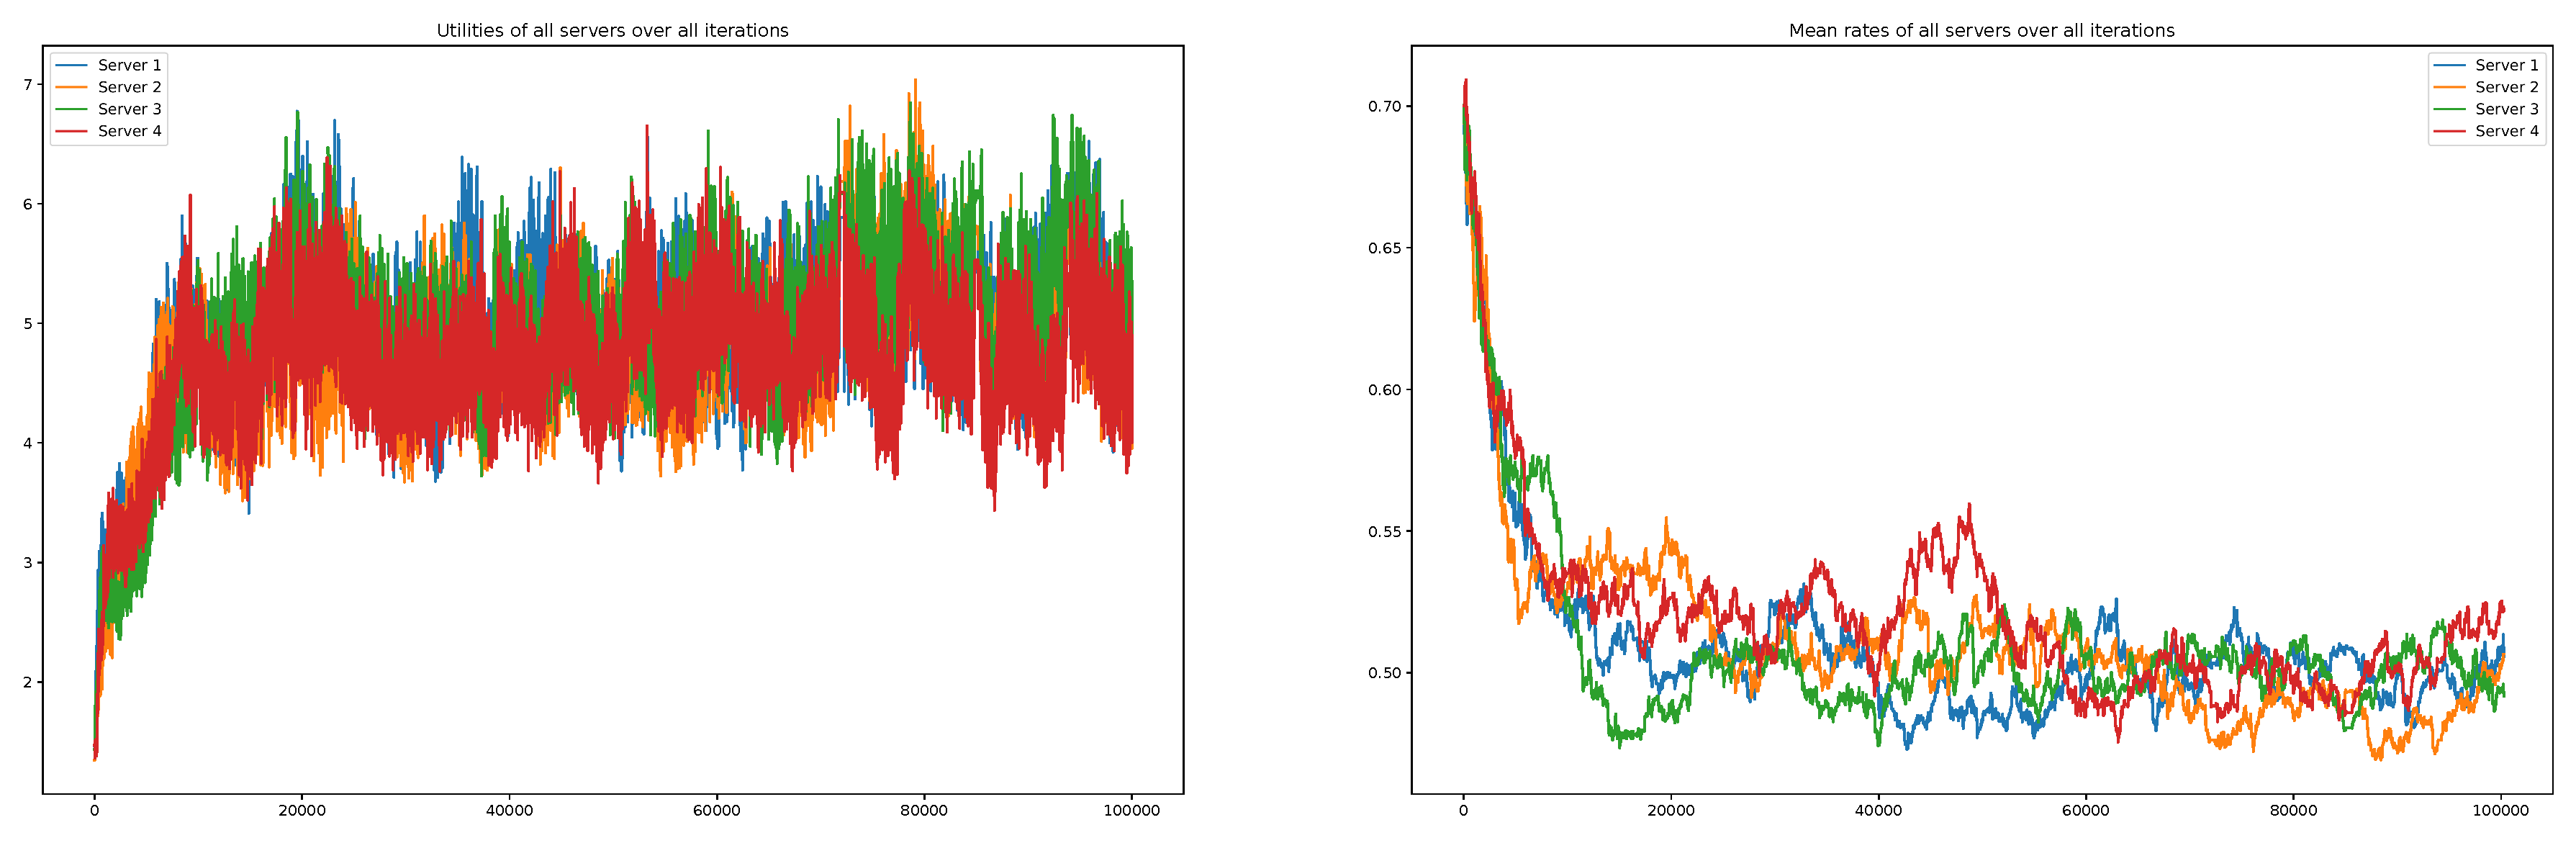
\includegraphics[width=\textwidth]{chapters/00_appendix/03_more_rl_results/Bin/utility_3_eps/u3_1_e1.eps}
    \caption{Utilities and mean service rate of servers from the reinforcement
    learning run using utility function \(U_k^{(3)}\) with \(e = 1\) and
    \(100000\) time steps}
    \label{fig:RL_utility3_1_e1}
\end{figure}

\begin{figure}[H]
    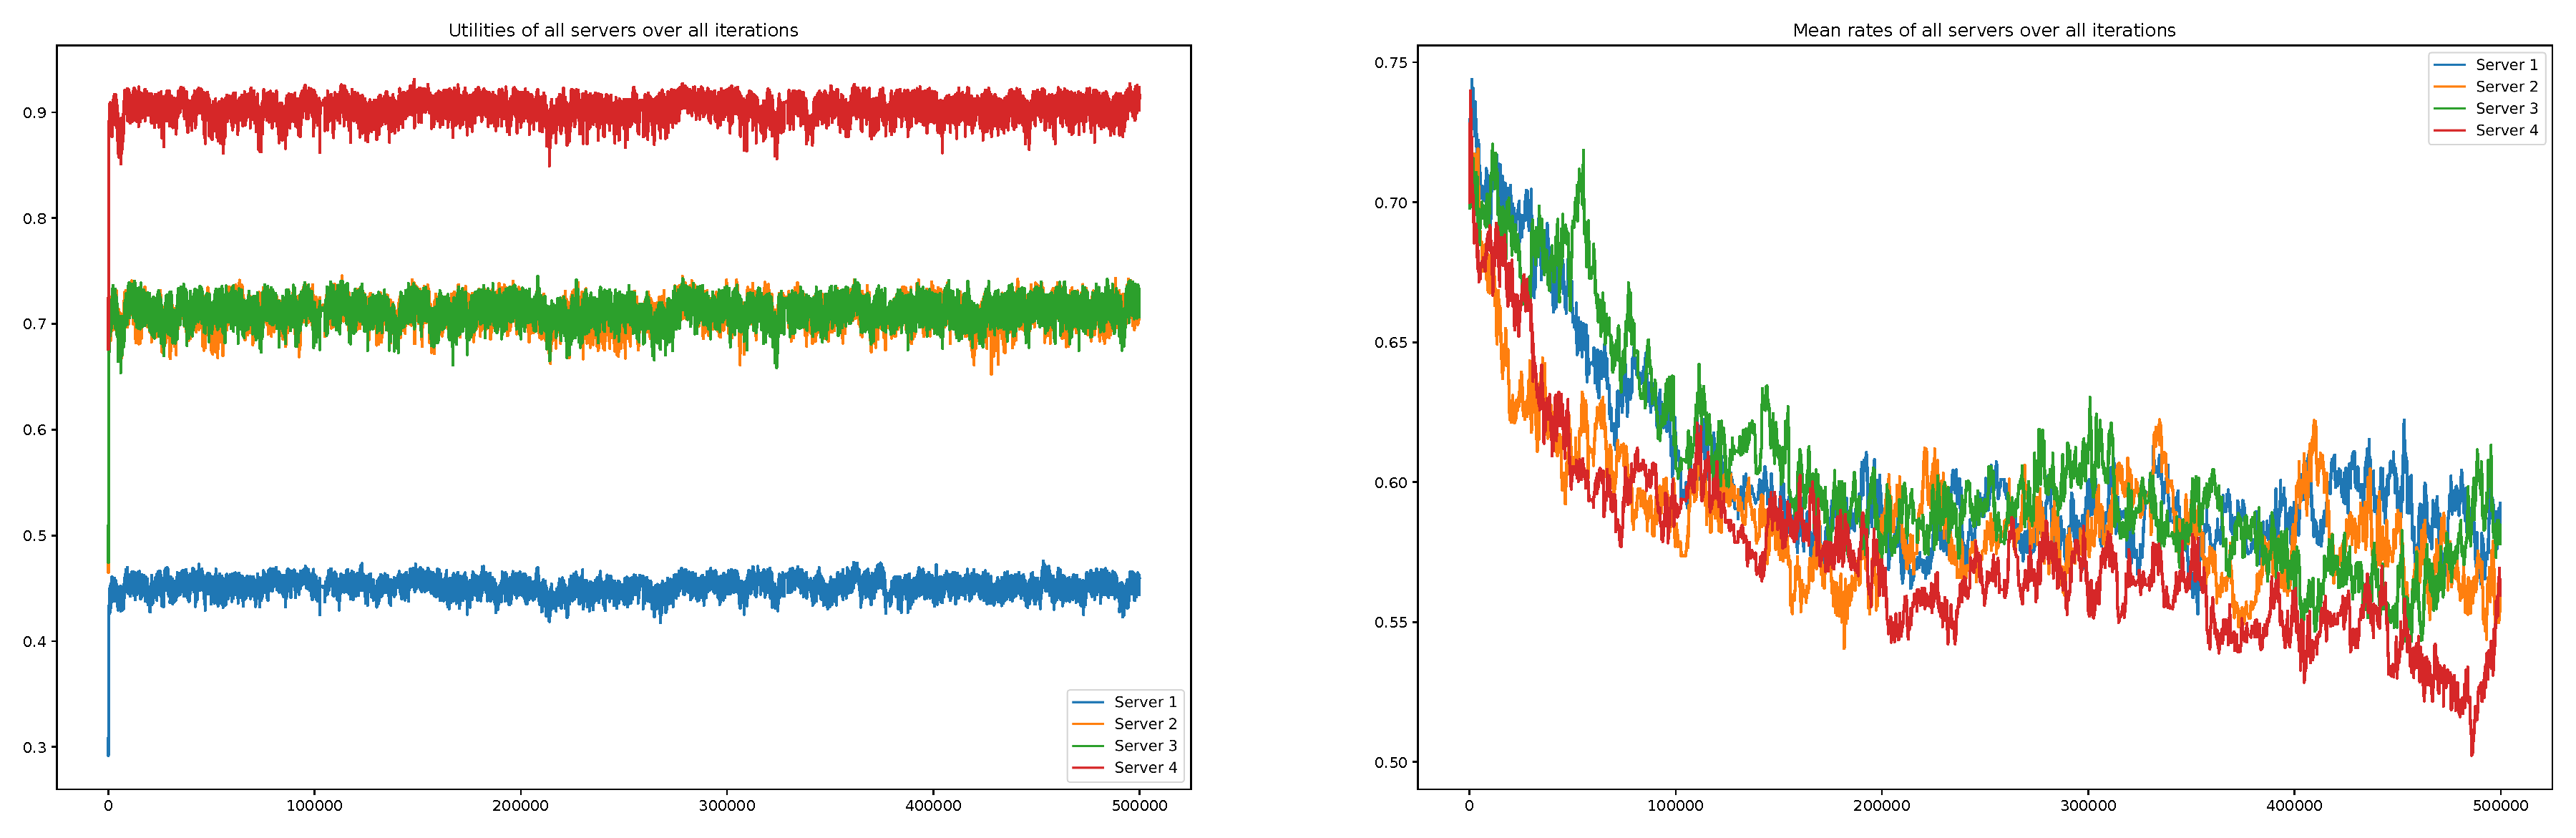
\includegraphics[width=\textwidth]{chapters/00_appendix/03_more_rl_results/Bin/utility_3_eps/u3_2_e0.eps}
    \caption{Utilities and mean service rate of servers from the reinforcement
    learning run using utility function \(U_k^{(3)}\) with \(e = 0\) and
    \(500000\) time steps}
    \label{fig:RL_utility3_2_e0}
\end{figure}

\begin{figure}[H]
    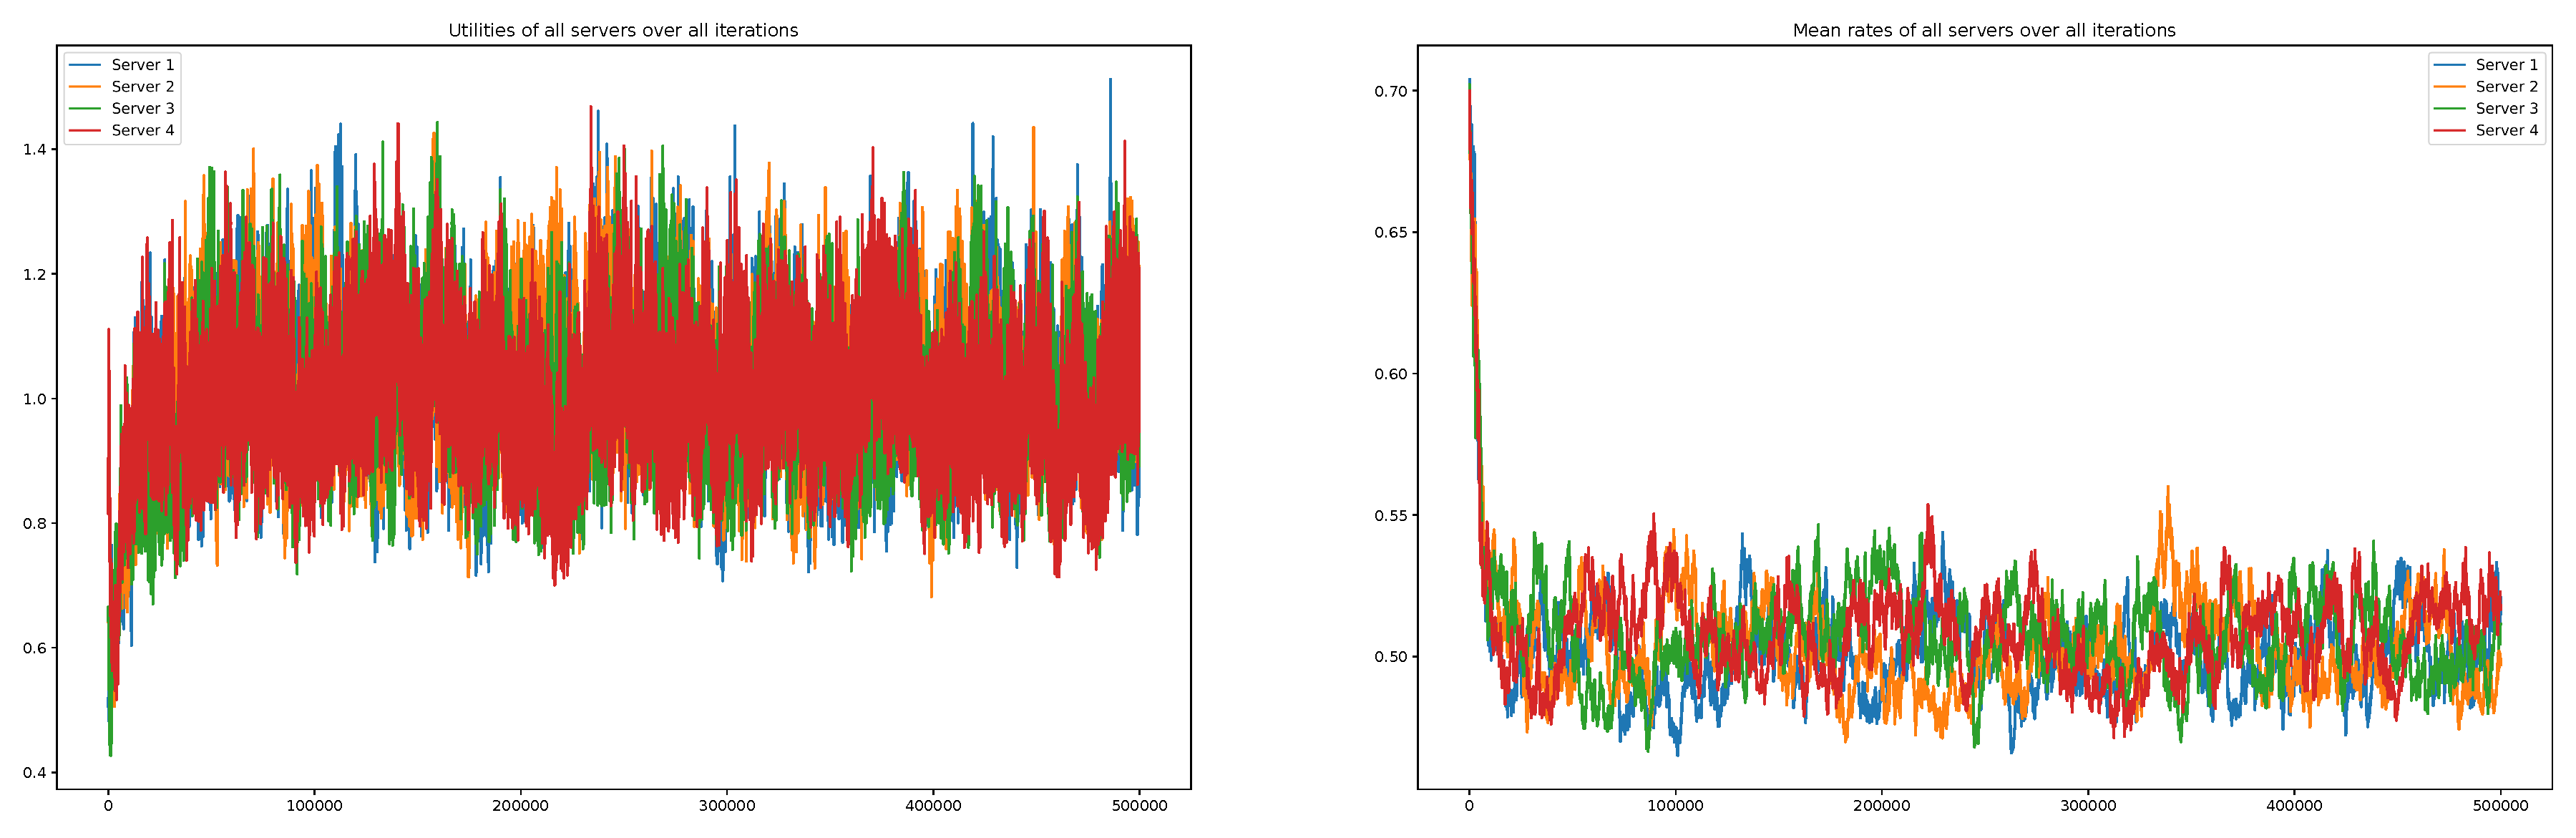
\includegraphics[width=\textwidth]{chapters/00_appendix/03_more_rl_results/Bin/utility_3_eps/u3_2_e02.eps}
    \caption{Utilities and mean service rate of servers from the reinforcement
    learning run using utility function \(U_k^{(3)}\) with \(e = 0.2\) and
    \(500000\) time steps}
    \label{fig:RL_utility3_2_e02}
\end{figure}

\begin{figure}[H]
    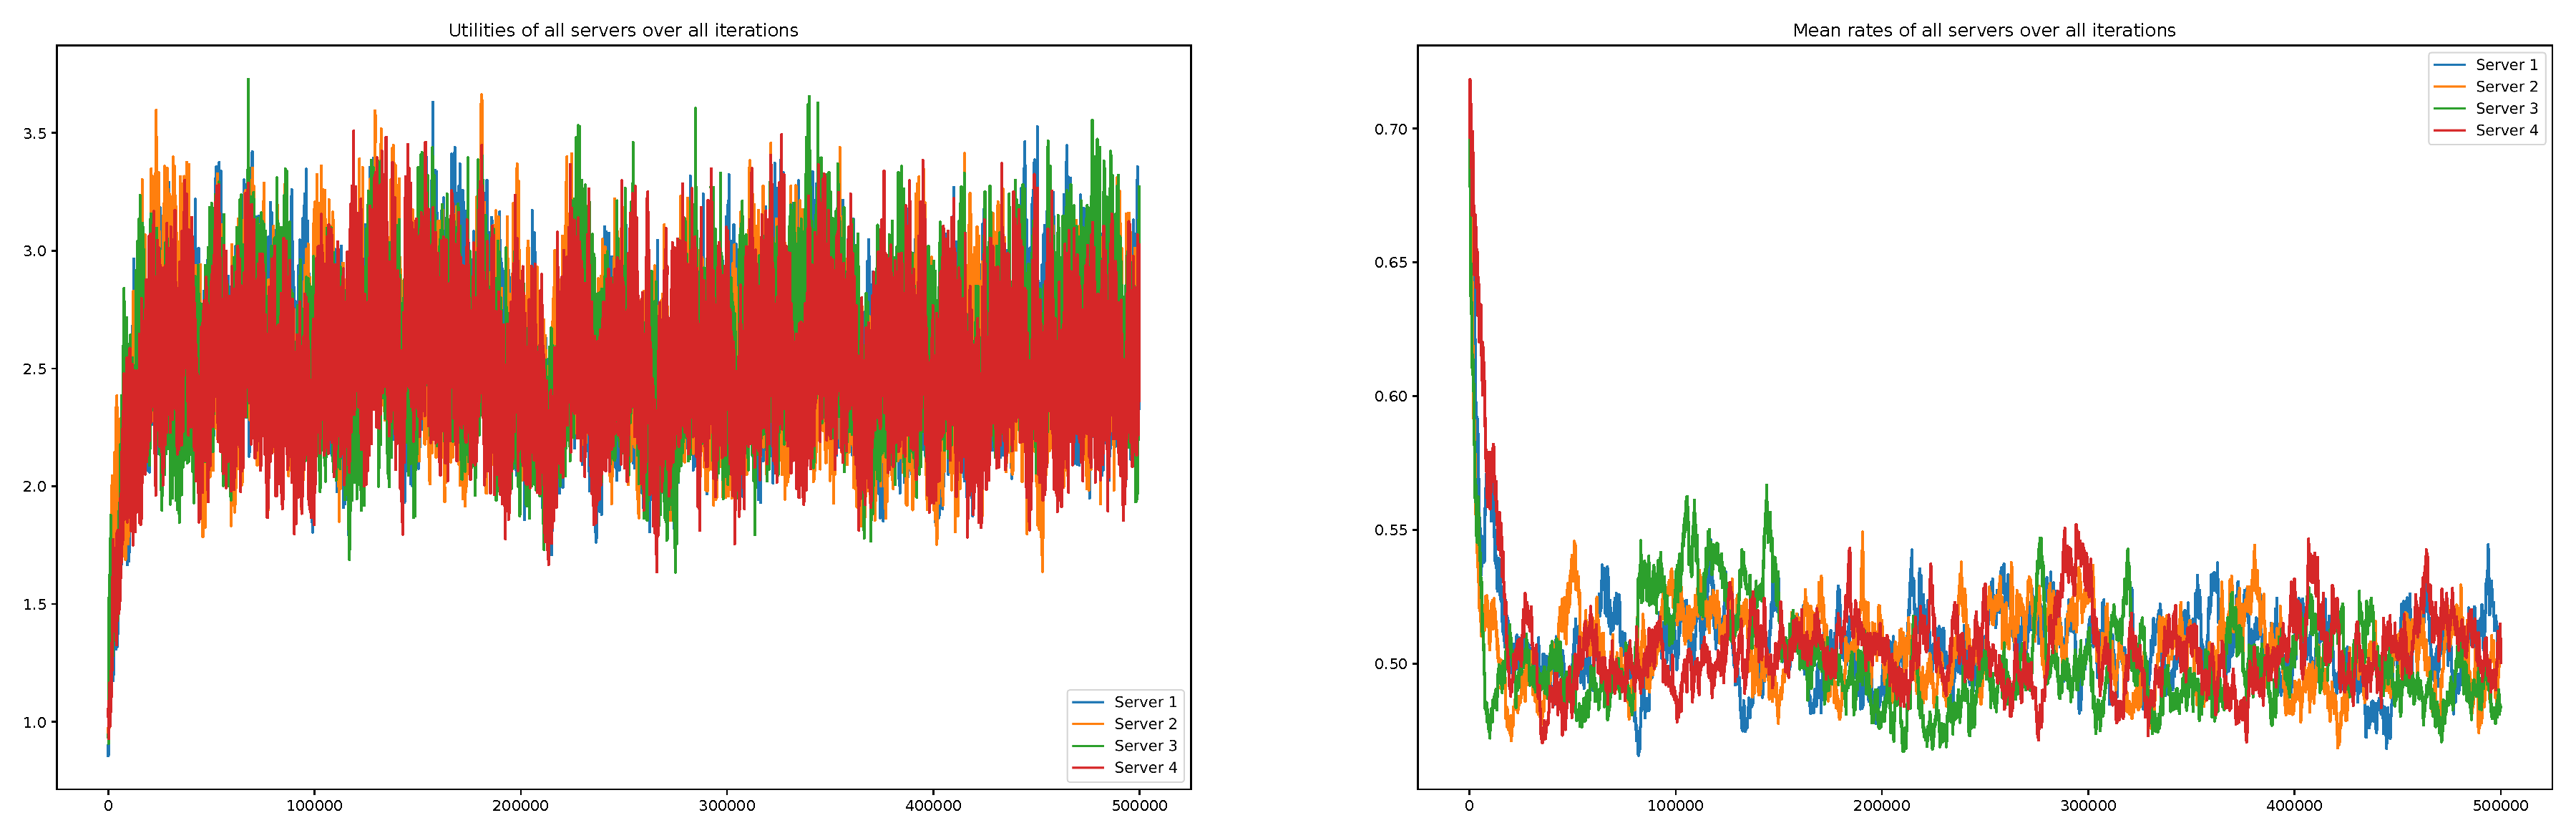
\includegraphics[width=\textwidth]{chapters/00_appendix/03_more_rl_results/Bin/utility_3_eps/u3_2_e05.eps}
    \caption{Utilities and mean service rate of servers from the reinforcement
    learning run using utility function \(U_k^{(3)}\) with \(e = 0.5\) and
    \(500000\) time steps}
    \label{fig:RL_utility3_2_e05}
\end{figure}

\begin{figure}[H]
    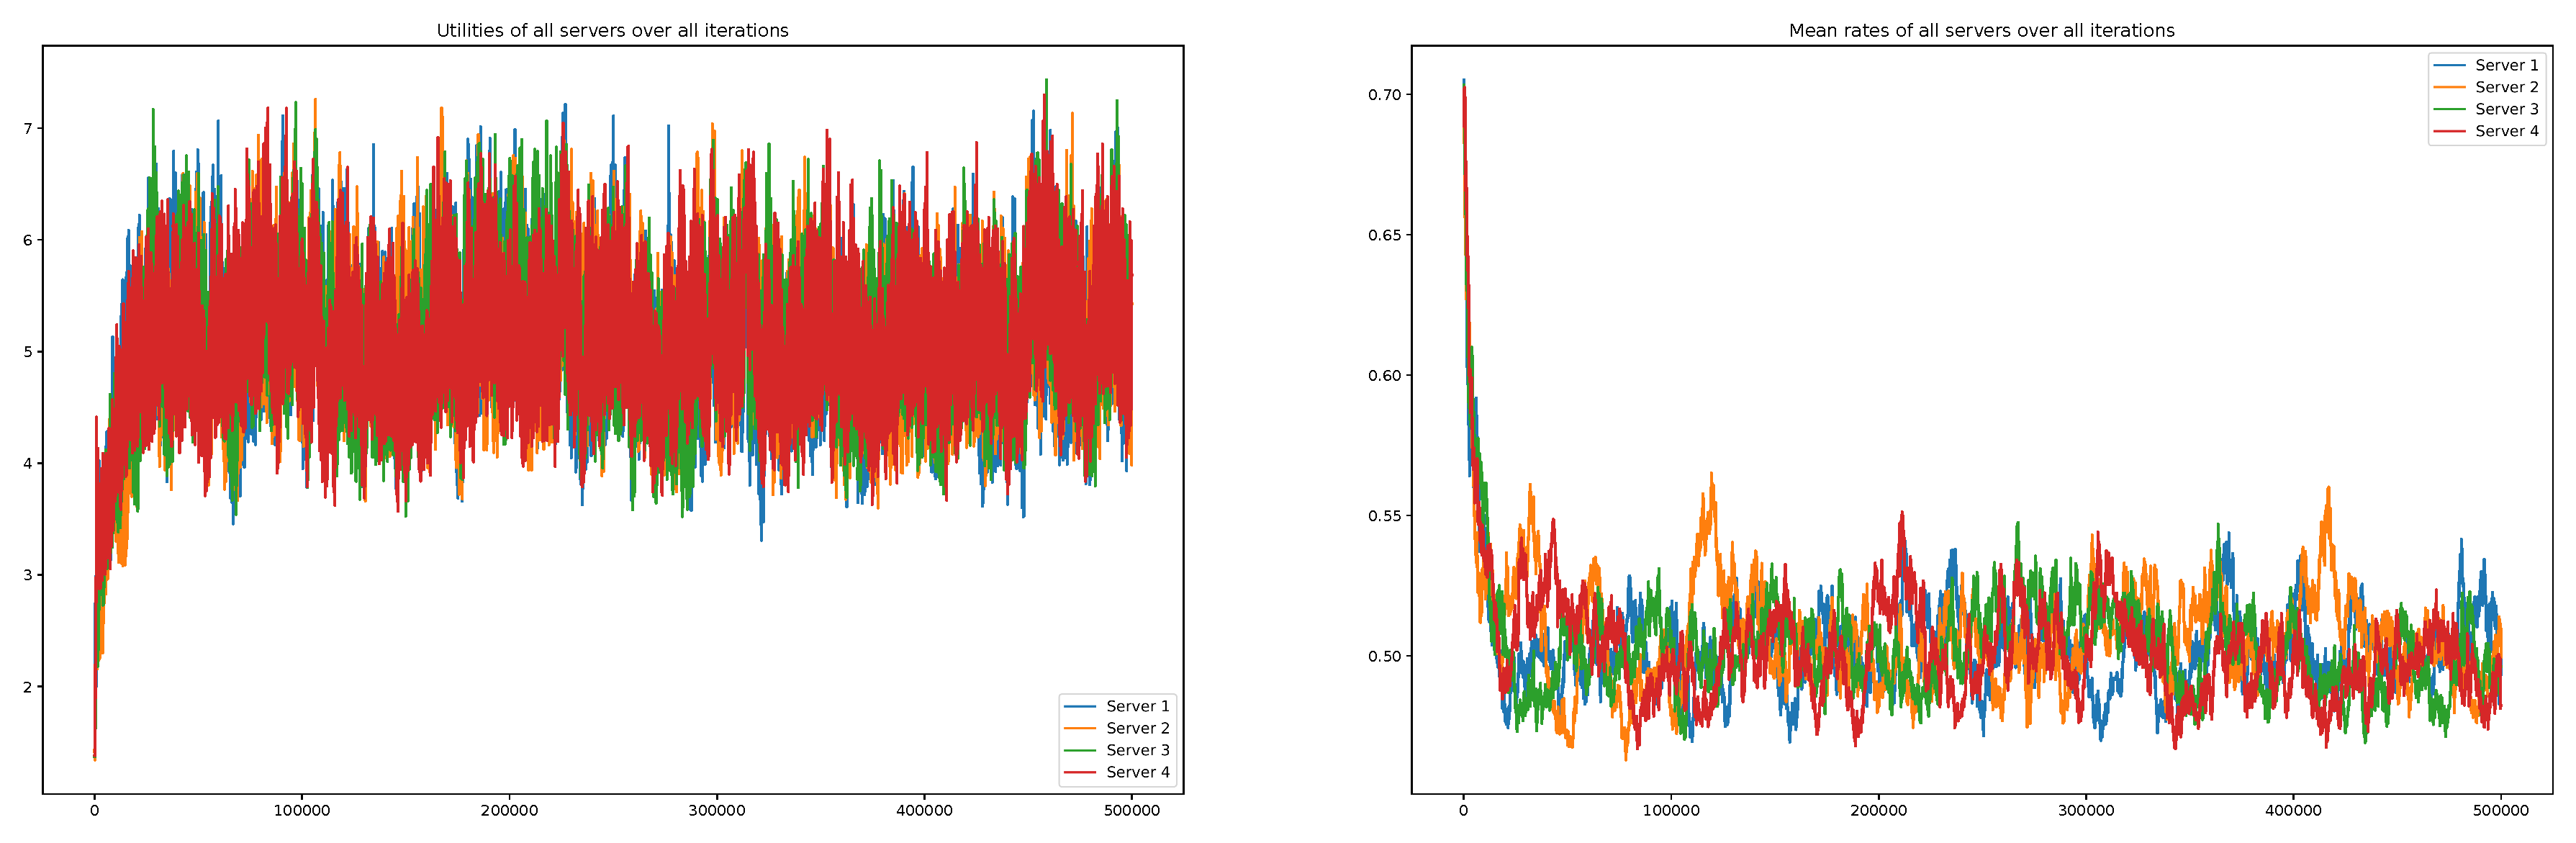
\includegraphics[width=\textwidth]{chapters/00_appendix/03_more_rl_results/Bin/utility_3_eps/u3_2_e1.eps}
    \caption{Utilities and mean service rate of servers from the reinforcement
    learning run using utility function \(U_k^{(3)}\) with \(e = 1\) and
    \(500000\) time steps}
    \label{fig:RL_utility3_2_e1}
\end{figure}

\begin{figure}[H]
    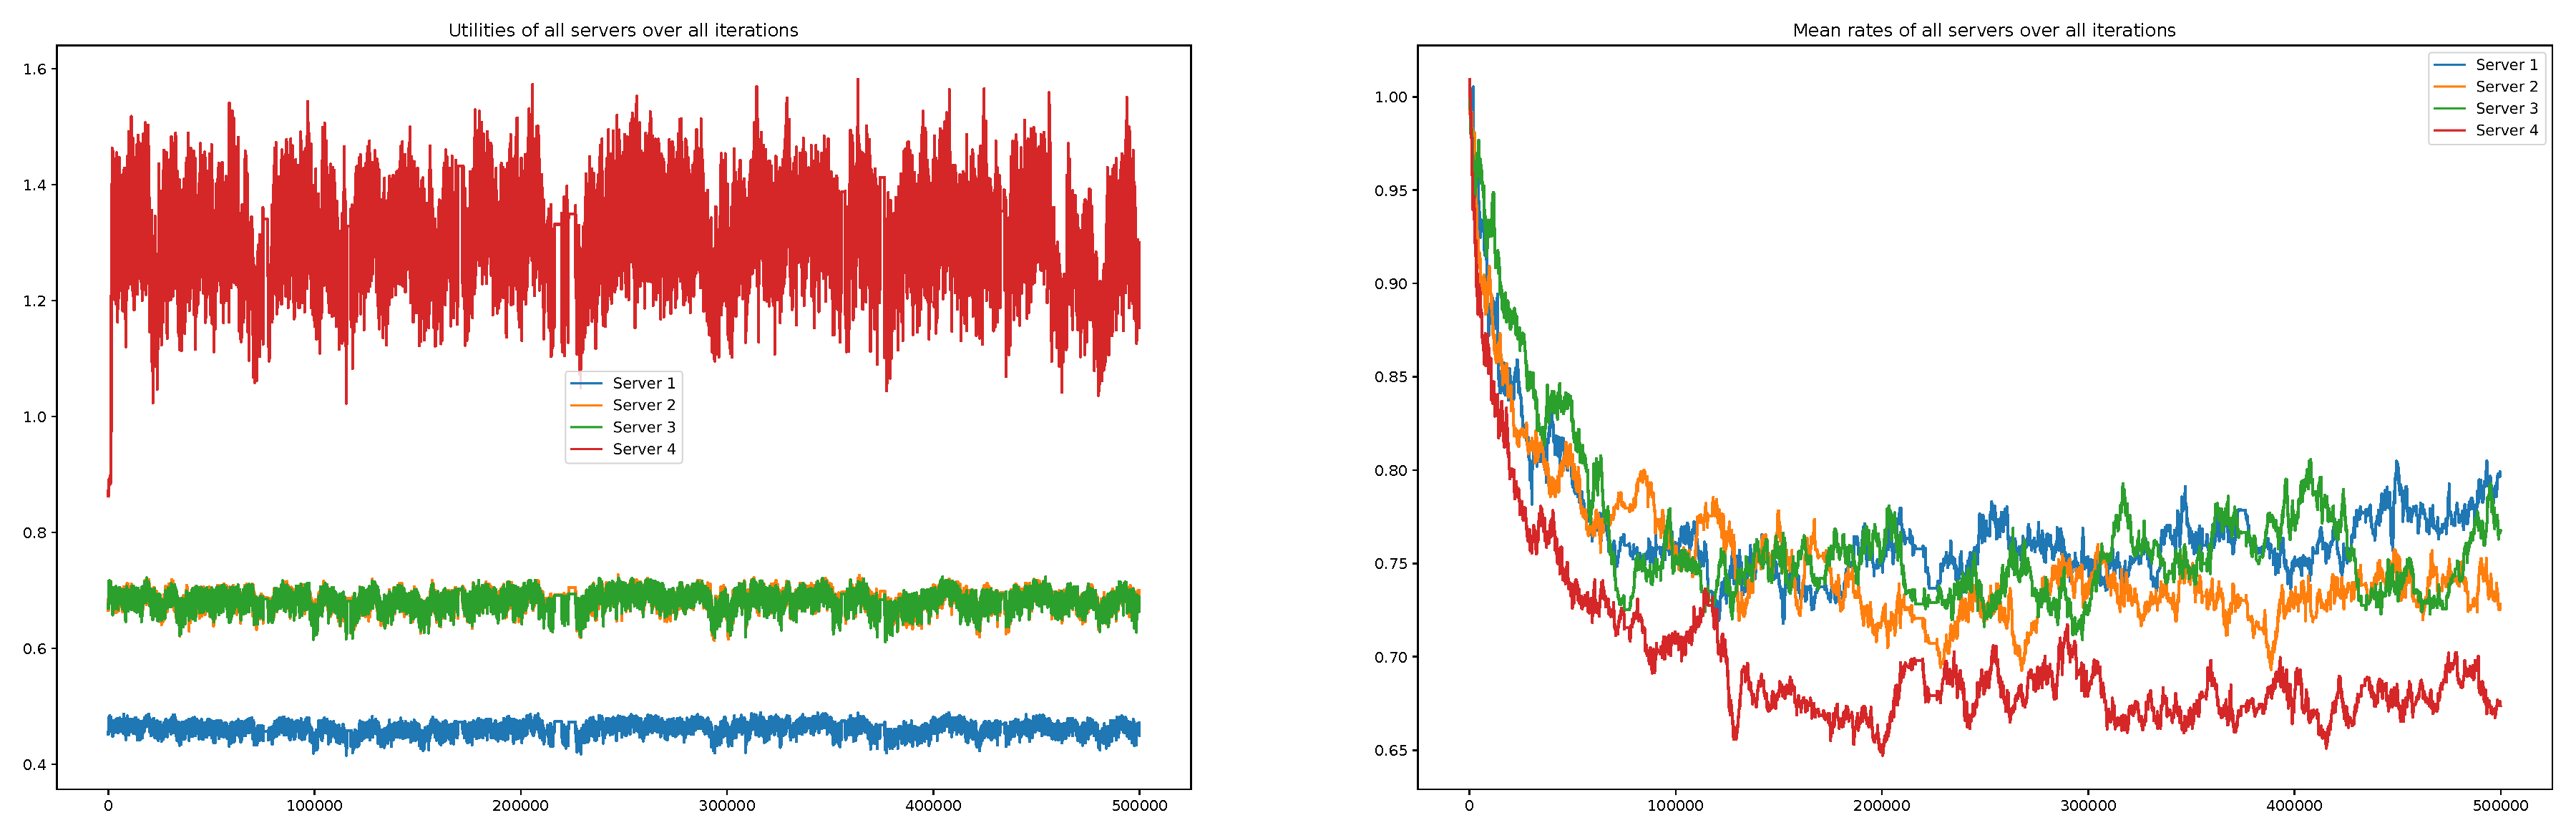
\includegraphics[width=\textwidth]{chapters/00_appendix/03_more_rl_results/Bin/utility_3_eps/u3_3_initial_1.eps}
    \caption{Utilities and mean service rate of servers from the reinforcement
    learning run using utility function \(U_k^{(3)}\) with \(e = 0.1\),
    \(500000\) time steps and an initial service rate of \(\mu = 1\) for all
    servers}
    \label{fig:RL_utility3_3_initial_1}
\end{figure}

\begin{figure}[H]
    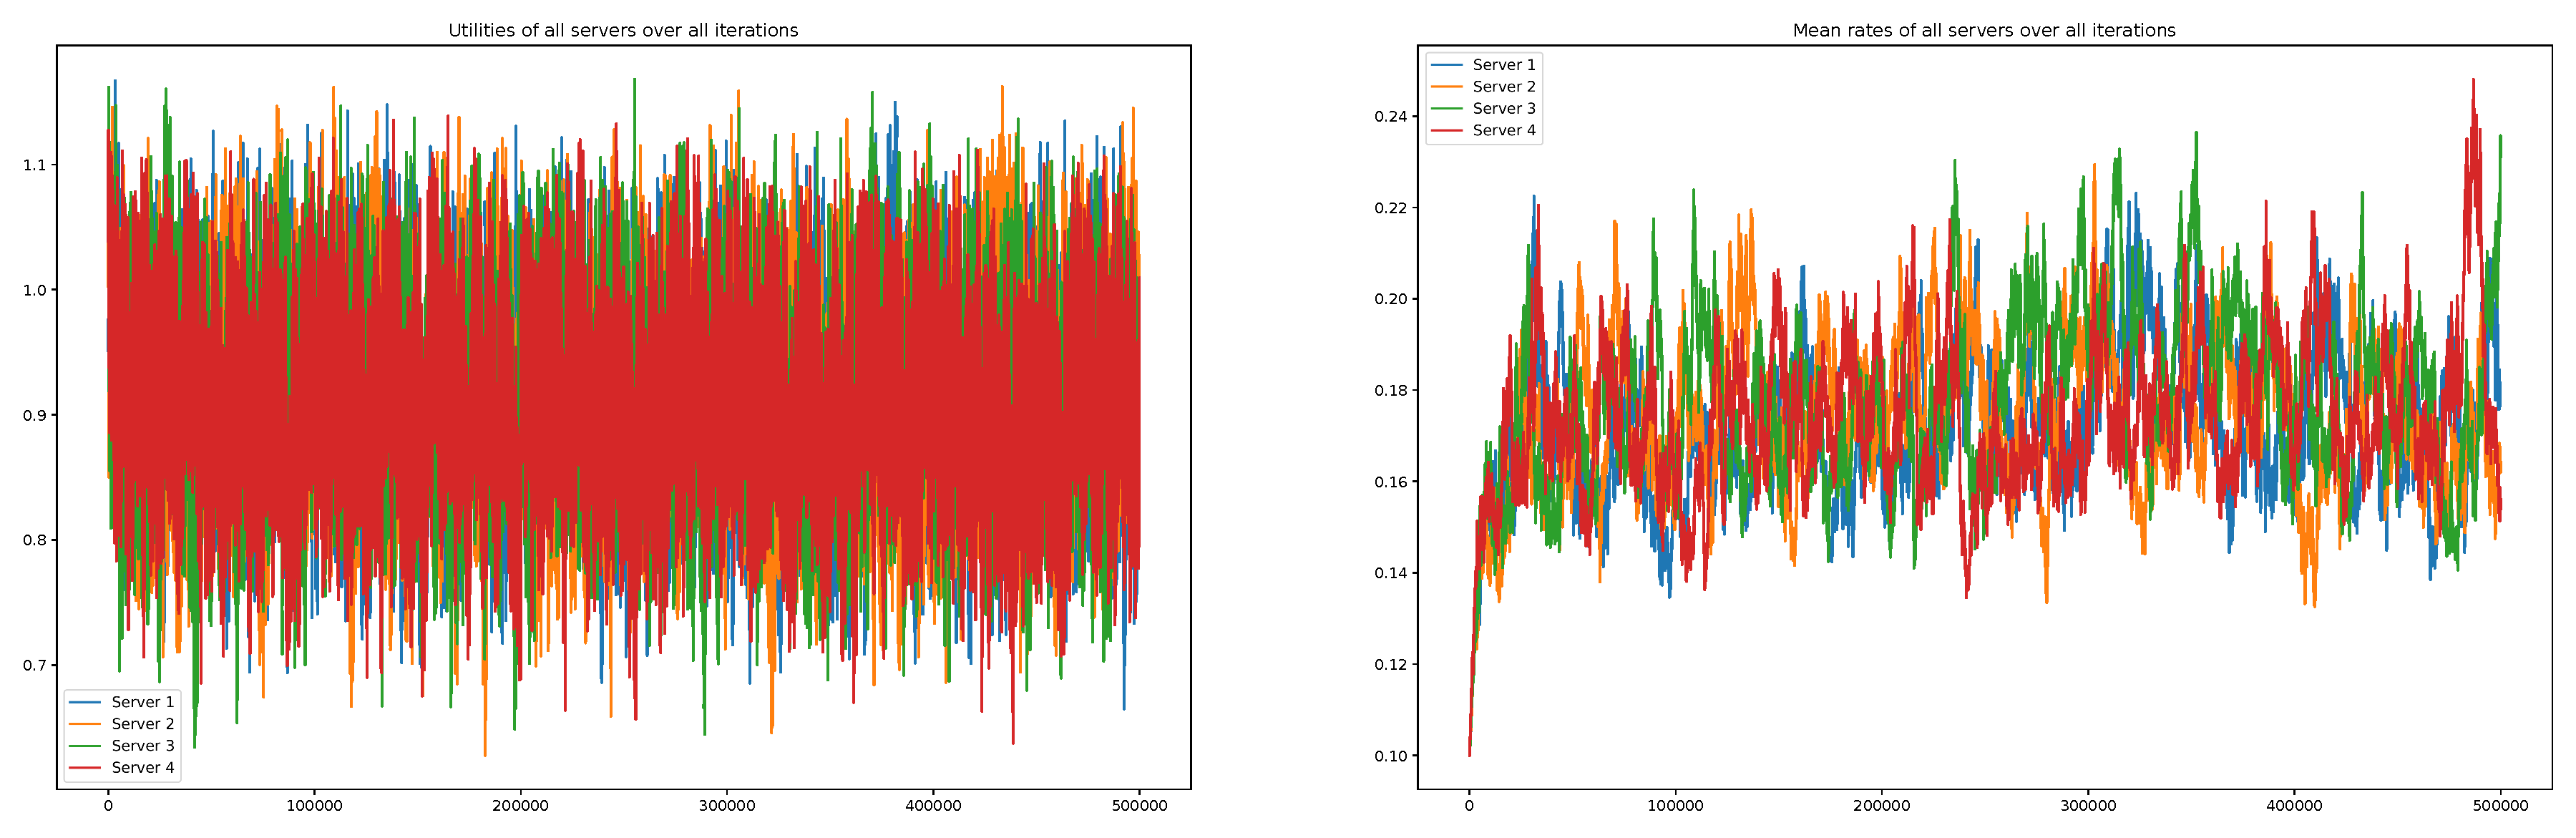
\includegraphics[width=\textwidth]{chapters/00_appendix/03_more_rl_results/Bin/utility_3_eps/u3_3_initial_01.eps}
    \caption{Utilities and mean service rate of servers from the reinforcement
    learning run using utility function \(U_k^{(3)}\) with \(e = 0.1\),
    \(500000\) time steps and an initial service rate of \(\mu = 0.1\) for all
    servers}
    \label{fig:RL_utility3_3_initial_01}
\end{figure}

\begin{figure}[H]
    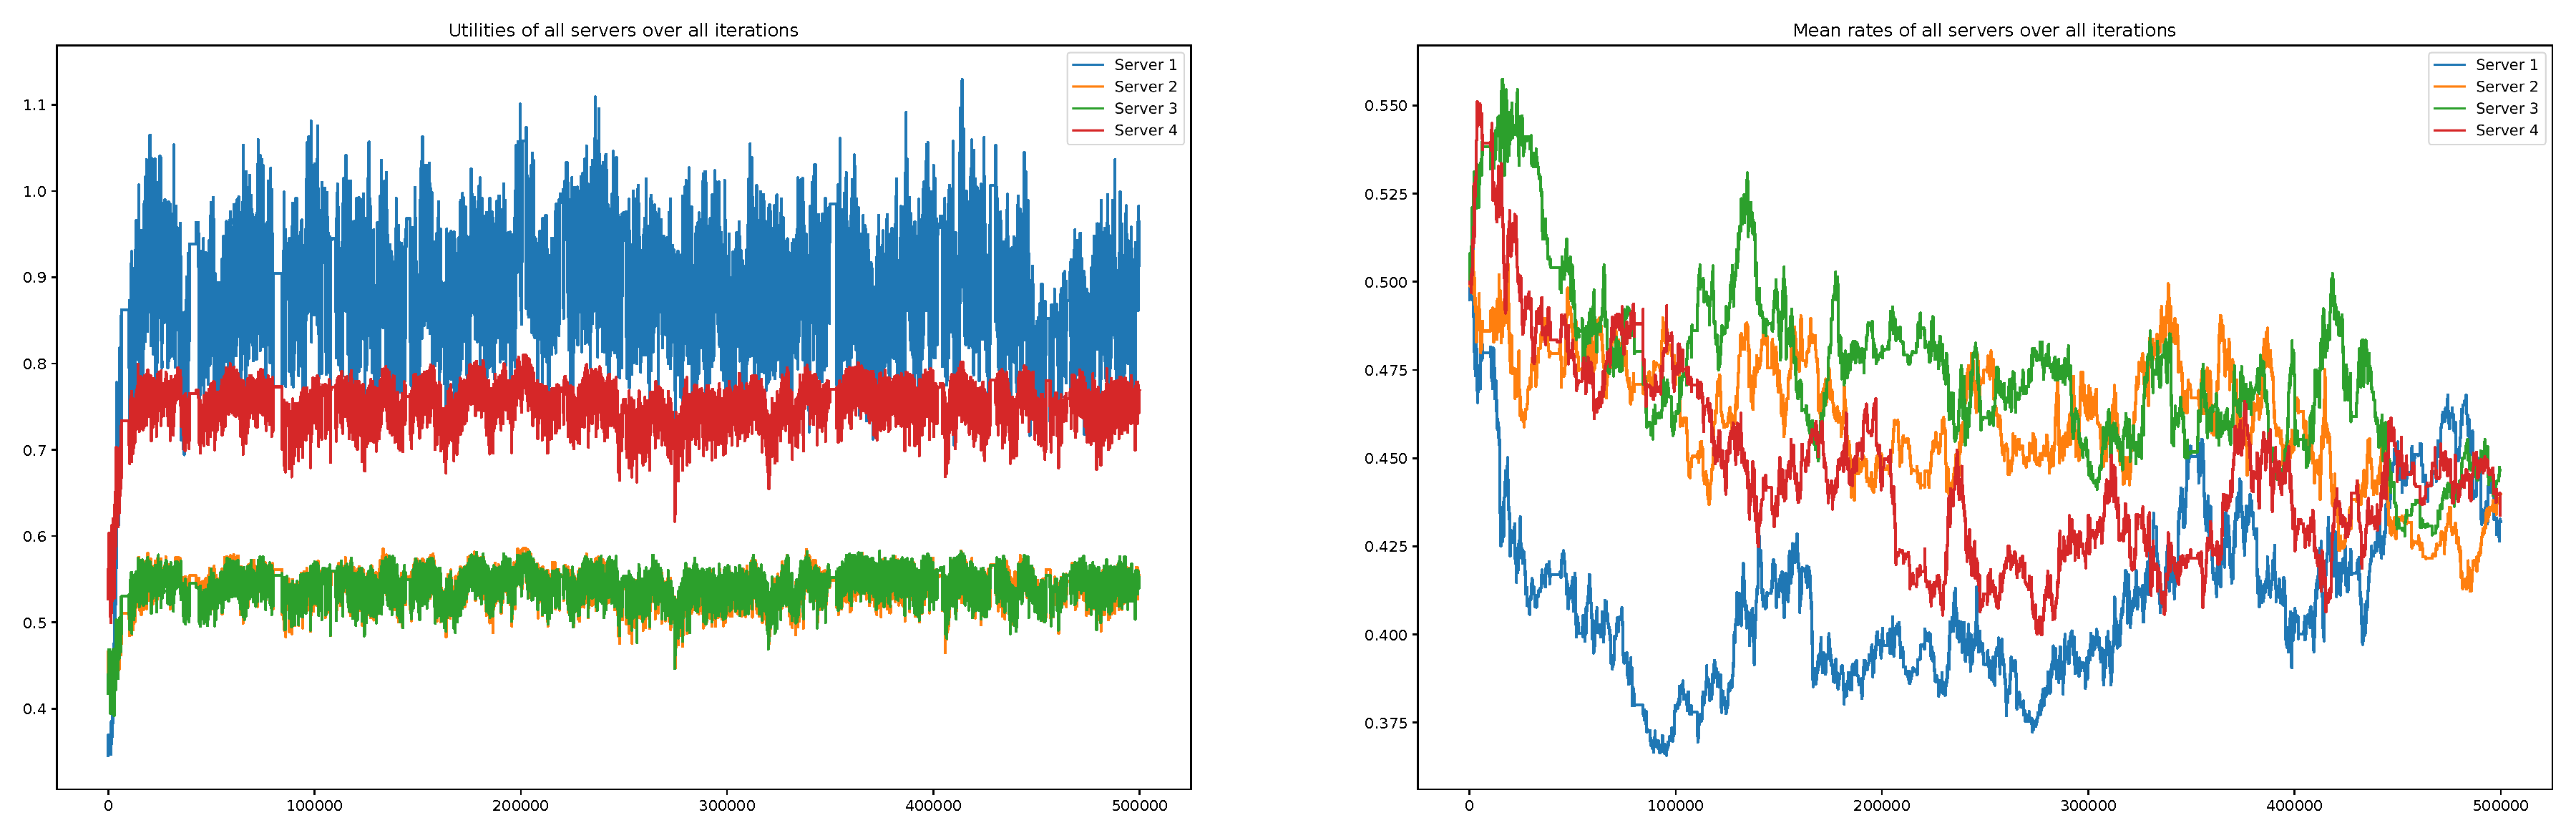
\includegraphics[width=\textwidth]{chapters/00_appendix/03_more_rl_results/Bin/utility_3_eps/u3_3_initial_05.eps}
    \caption{Utilities and mean service rate of servers from the reinforcement
    learning run using utility function \(U_k^{(3)}\) with \(e = 0.1\),
    \(500000\) time steps and an initial service rate of \(\mu = 0.5\) for all
    servers}
    \label{fig:RL_utility3_3_initial_05}
\end{figure}

\begin{figure}[H]
    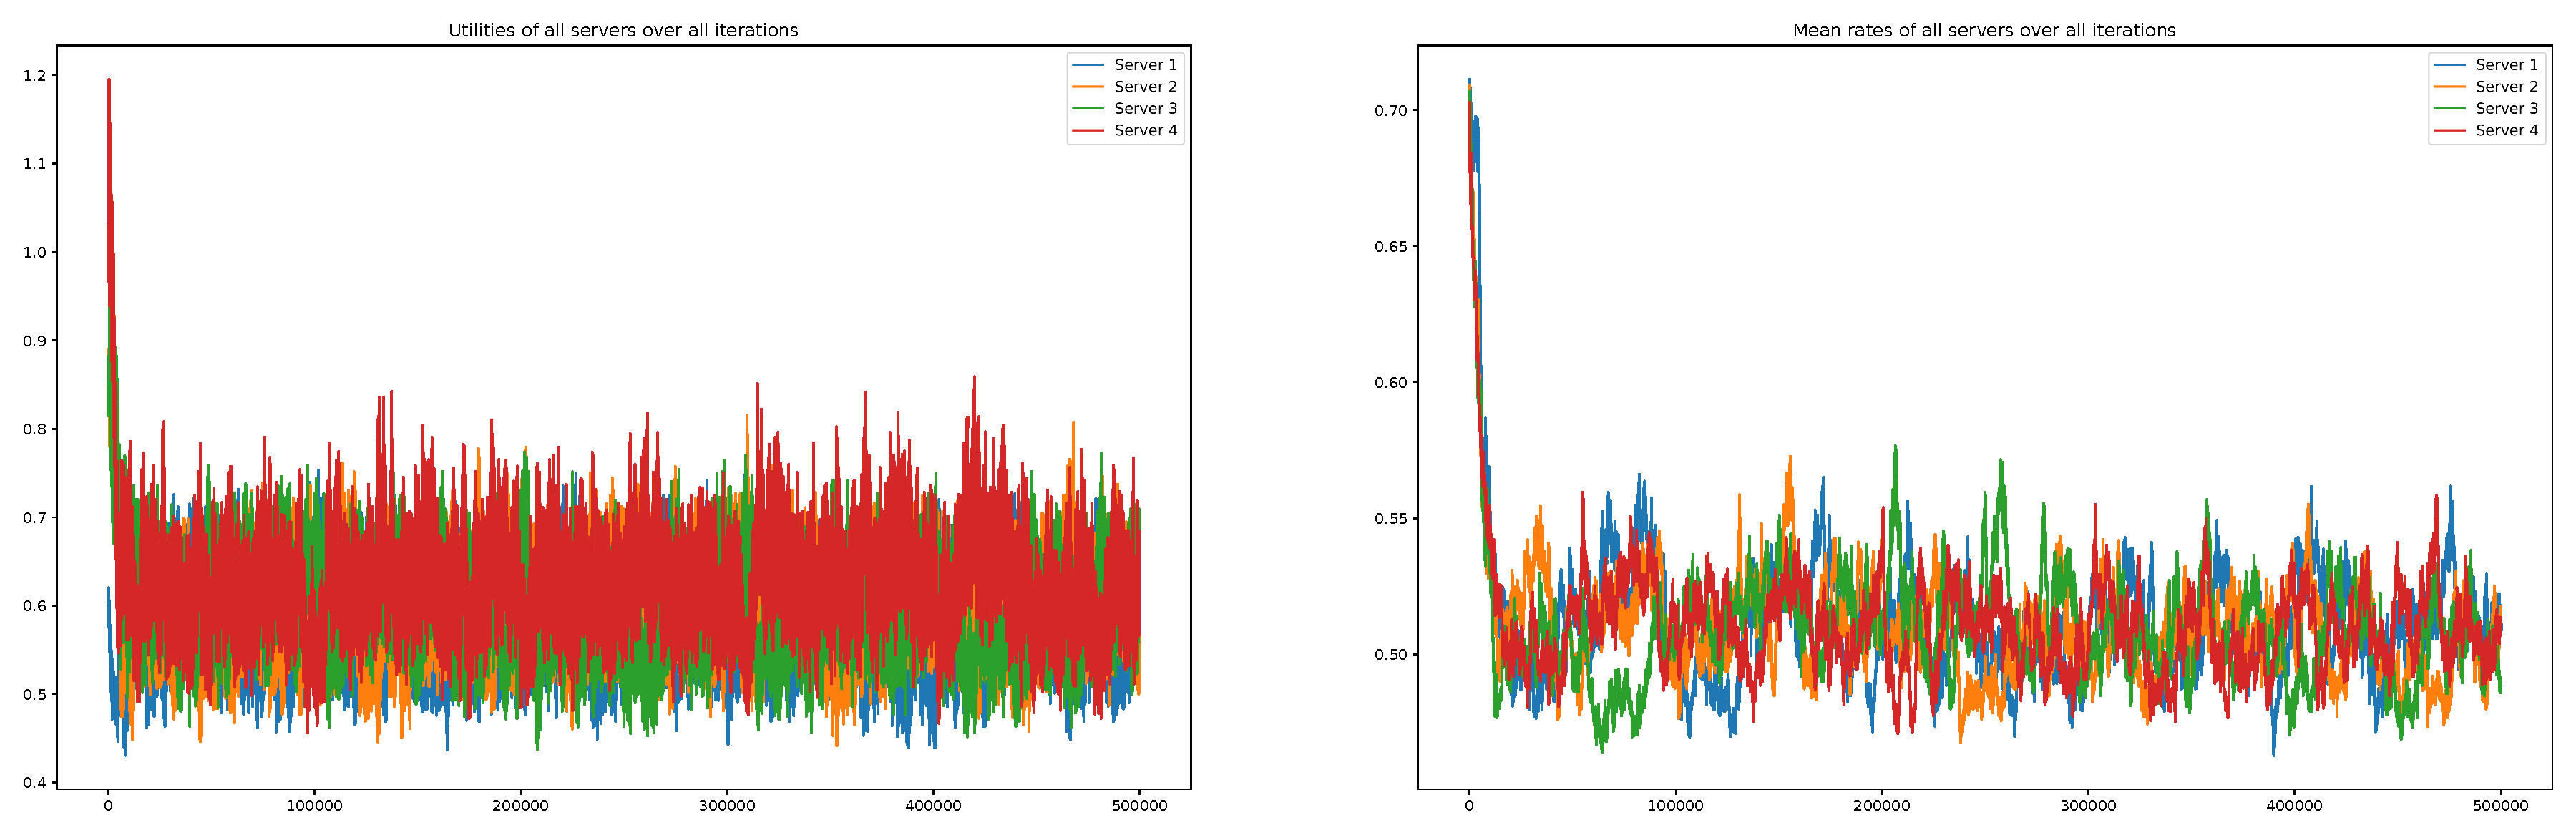
\includegraphics[width=\textwidth]{chapters/00_appendix/03_more_rl_results/Bin/utility_3_eps/u3_4_lambda2_05.eps}
    \caption{Utilities and mean service rate of servers from the reinforcement
    learning run using utility function \(U_k^{(3)}\) with \(e = 1\) and
    \(500000\) time steps decreasing \(\lambda_2\) to \(0.5\)}
    \label{fig:RL_utility3_4_lambda2_05}
\end{figure}

\begin{figure}[H]
    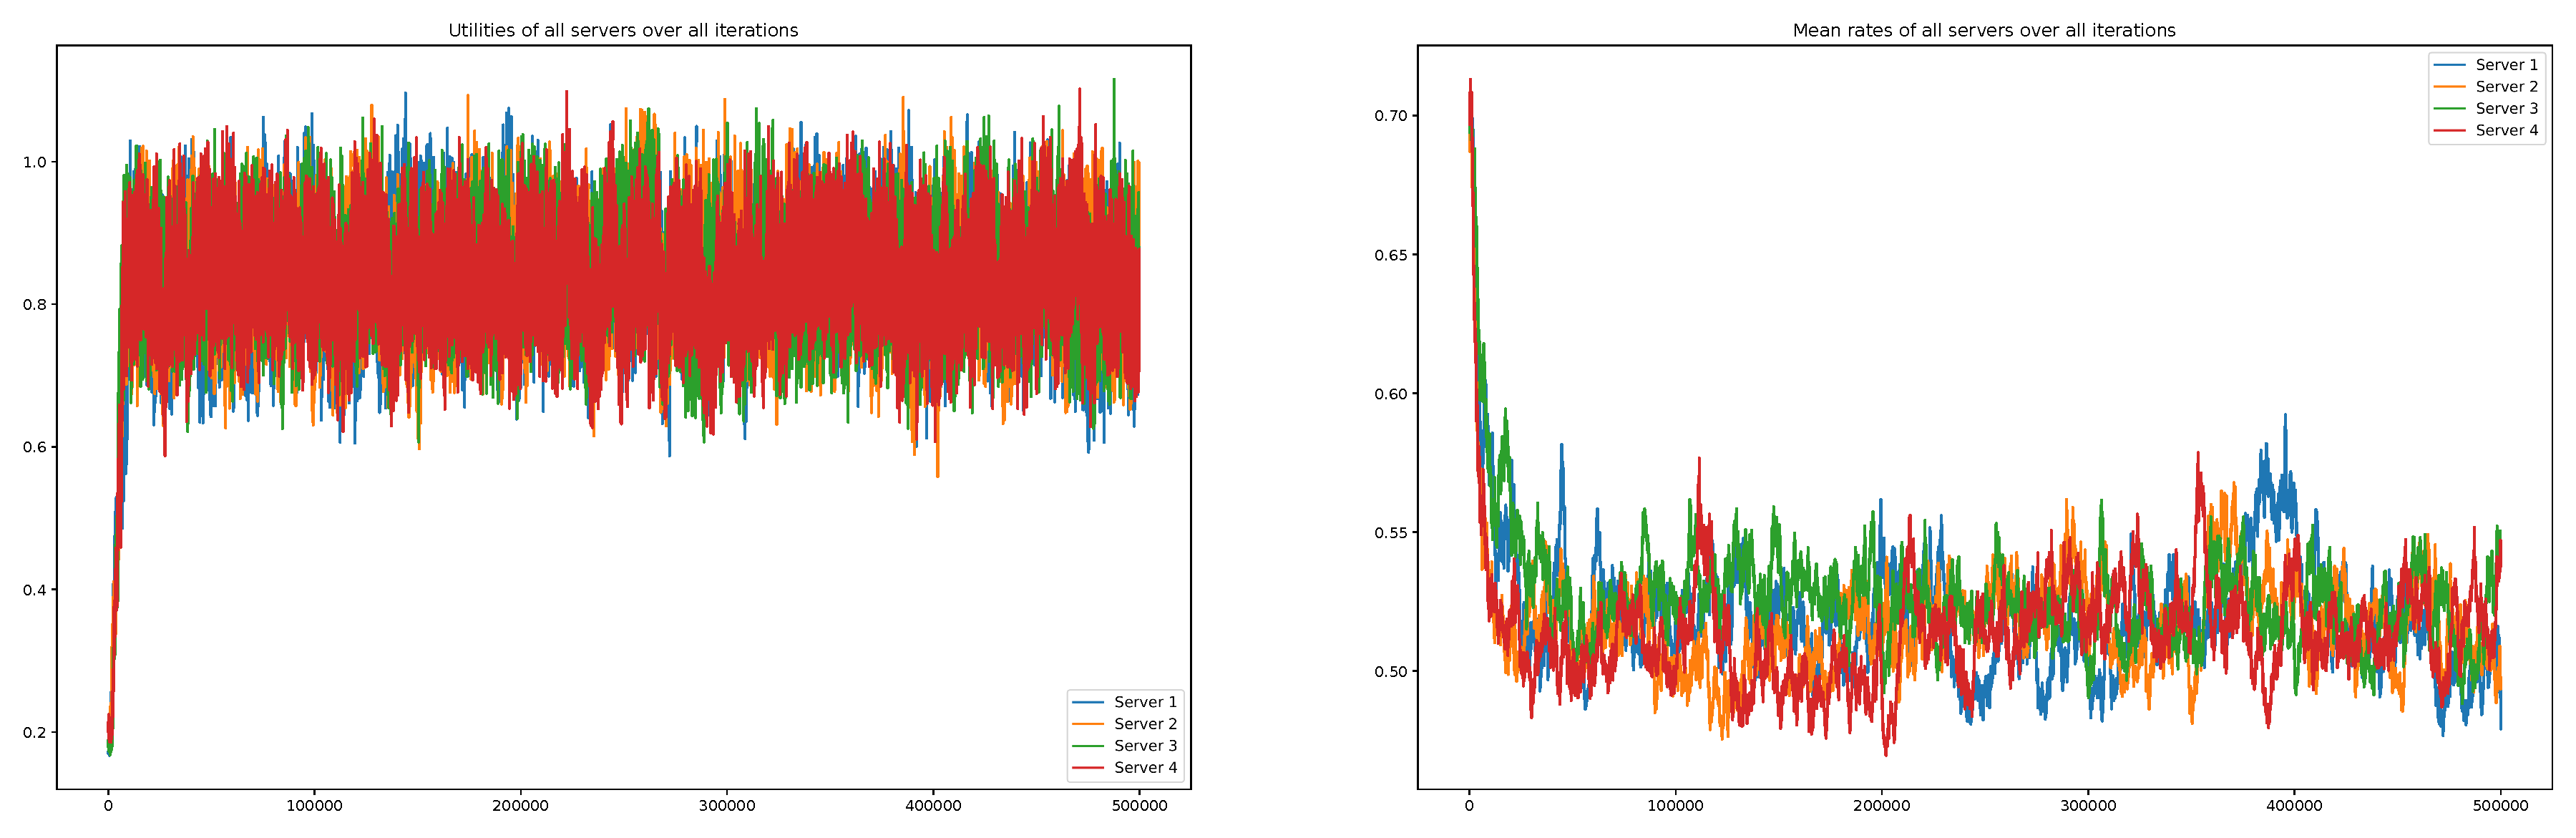
\includegraphics[width=\textwidth]{chapters/00_appendix/03_more_rl_results/Bin/utility_3_eps/u3_4_lambda2_15.eps}
    \caption{Utilities and mean service rate of servers from the reinforcement
    learning run using utility function \(U_k^{(3)}\) with \(e = 1\) and
    \(500000\) time steps increasing \(\lambda_2\) to \(1.5\)}
    \label{fig:RL_utility3_4_lambda2_15}
\end{figure}

% u7_1_e0.pdf
\begin{figure}[H]
    \includegraphics[width=\textwidth]{chapters/00_appendix/03_more_rl_results/Bin/utility_7/u7_1_e0.pdf}
    \caption{Utilities and mean service rate of servers from the reinforcement
    learning run using utility function \(U_k^{(7)}\) with \(e = 0\).}
    \label{fig:RL_utility7_1_e0}
\end{figure}

% u7_1_e01.pdf
\begin{figure}[H]
    \includegraphics[width=\textwidth]{chapters/00_appendix/03_more_rl_results/Bin/utility_7/u7_1_e01.pdf}
    \caption{Utilities and mean service rate of servers from the reinforcement
    learning run using utility function \(U_k^{(7)}\) with \(e = 0.1\).}
    \label{fig:RL_utility7_1_e01}
\end{figure}

% u7_1_e02.pdf
\begin{figure}[H]
    \includegraphics[width=\textwidth]{chapters/00_appendix/03_more_rl_results/Bin/utility_7/u7_1_e02.pdf}
    \caption{Utilities and mean service rate of servers from the reinforcement
    learning run using utility function \(U_k^{(7)}\) with \(e = 0.2\).}
    \label{fig:RL_utility7_1_e02}
\end{figure}

% u7_1_e03.pdf
\begin{figure}[H]
    \includegraphics[width=\textwidth]{chapters/00_appendix/03_more_rl_results/Bin/utility_7/u7_1_e03.pdf}
    \caption{Utilities and mean service rate of servers from the reinforcement
    learning run using utility function \(U_k^{(7)}\) with \(e = 0.3\).}
    \label{fig:RL_utility7_1_e03}
\end{figure}

% u7_1_e04.pdf
\begin{figure}[H]
    \includegraphics[width=\textwidth]{chapters/00_appendix/03_more_rl_results/Bin/utility_7/u7_1_e04.pdf}
    \caption{Utilities and mean service rate of servers from the reinforcement
    learning run using utility function \(U_k^{(7)}\) with \(e = 0.4\).}
    \label{fig:RL_utility7_1_e04}
\end{figure}

% u7_1_e05.pdf
\begin{figure}[H]
    \includegraphics[width=\textwidth]{chapters/00_appendix/03_more_rl_results/Bin/utility_7/u7_1_e05.pdf}
    \caption{Utilities and mean service rate of servers from the reinforcement
    learning run using utility function \(U_k^{(7)}\) with \(e = 0.5\).}
    \label{fig:RL_utility7_1_e05}
\end{figure}

% u7_1_e06.pdf
\begin{figure}[H]
    \includegraphics[width=\textwidth]{chapters/00_appendix/03_more_rl_results/Bin/utility_7/u7_1_e06.pdf}
    \caption{Utilities and mean service rate of servers from the reinforcement
    learning run using utility function \(U_k^{(7)}\) with \(e = 0.6\).}
    \label{fig:RL_utility7_1_e06}
\end{figure}

% u7_1_e07.pdf
\begin{figure}[H]
    \includegraphics[width=\textwidth]{chapters/00_appendix/03_more_rl_results/Bin/utility_7/u7_1_e07.pdf}
    \caption{Utilities and mean service rate of servers from the reinforcement
    learning run using utility function \(U_k^{(7)}\) with \(e = 0.7\).}
    \label{fig:RL_utility7_1_e07}
\end{figure}

% u7_1_e08.pdf
\begin{figure}[H]
    \includegraphics[width=\textwidth]{chapters/00_appendix/03_more_rl_results/Bin/utility_7/u7_1_e08.pdf}
    \caption{Utilities and mean service rate of servers from the reinforcement
    learning run using utility function \(U_k^{(7)}\) with \(e = 0.8\).}
    \label{fig:RL_utility7_1_e08}
\end{figure}

% u7_1_e09.pdf
\begin{figure}[H]
    \includegraphics[width=\textwidth]{chapters/00_appendix/03_more_rl_results/Bin/utility_7/u7_1_e09.pdf}
    \caption{Utilities and mean service rate of servers from the reinforcement
    learning run using utility function \(U_k^{(7)}\) with \(e = 0.9\).}
    \label{fig:RL_utility7_1_e09}
\end{figure}

% u7_1_e1.pdf
\begin{figure}[H]
    \includegraphics[width=\textwidth]{chapters/00_appendix/03_more_rl_results/Bin/utility_7/u7_1_e1.pdf}
    \caption{Utilities and mean service rate of servers from the reinforcement
    learning run using utility function \(U_k^{(7)}\) with \(e = 1\).}
    \label{fig:RL_utility7_1_e1}
\end{figure}

% u7_2_e01_early_iter.pdf
\begin{figure}[H]
    \includegraphics[width=\textwidth]{chapters/00_appendix/03_more_rl_results/Bin/utility_7/u7_2_e01_early_iter.pdf}
    \caption{Utilities and mean service rate of servers from the reinforcement
    learning run using utility function \(U_k^{(7)}\) with \(e = 0.1\) (only
    the early iterations)}
    \label{fig:RL_utility7_2_e01_early_iter}
\end{figure}

% u7_2_e01_late_iter.pdf
\begin{figure}[H]
    \includegraphics[width=\textwidth]{chapters/00_appendix/03_more_rl_results/Bin/utility_7/u7_2_e01_late_iter.pdf}
    \caption{Utilities and mean service rate of servers from the reinforcement
    learning run using utility function \(U_k^{(7)}\) with \(e = 0.1\) (only
    the late iterations)}
    \label{fig:RL_utility7_2_e01_late_iter}
\end{figure}

% u7_3_e01_markov.pdf
\begin{figure}[H]
    \includegraphics[width=\textwidth]{chapters/00_appendix/03_more_rl_results/Bin/utility_7/u7_3_e01_markov.pdf}
    \caption{Utilities and approximation of the weighted mean service rate of
    servers from the reinforcement learning run using utility function
    \(U_k^{(7)}\) with \(e = 0.1\). Note that the approximation uses the Markov
    chain model to get the state probabilities instead of the DES state
    probabilities.}
    \label{fig:RL_utility7_3_e01_markov}
\end{figure}

% u7_3_e05_markov.pdf
\begin{figure}[H]
    \includegraphics[width=\textwidth]{chapters/00_appendix/03_more_rl_results/Bin/utility_7/u7_3_e05_markov.pdf}
    \caption{Utilities and approximation of the weighted mean service rate of
    servers from the reinforcement learning run using utility function
    \(U_k^{(7)}\) with \(e = 0.5\). Note that the approximation uses the Markov
    chain model to get the state probabilities instead of the DES state
    probabilities.}
    \label{fig:RL_utility7_3_e05_markov}
\end{figure}

% u7_3_e09_markov.pdf
\begin{figure}[H]
    \includegraphics[width=\textwidth]{chapters/00_appendix/03_more_rl_results/Bin/utility_7/u7_3_e09_markov.pdf}
    \caption{Utilities and approximation of the weighted mean service rate of
    servers from the reinforcement learning run using utility function
    \(U_k^{(7)}\) with \(e = 0.9\). Note that the approximation uses the Markov
    chain model to get the state probabilities instead of the DES state
    probabilities.}
    \label{fig:RL_utility7_3_e09_markov}
\end{figure}


% u7_4_e01_Lambda_25.pdf
\begin{figure}[H]
    \includegraphics[width=\textwidth]{chapters/00_appendix/03_more_rl_results/Bin/utility_7/u7_4_e01_Lambda_25.pdf}
    \caption{Utilities and mean service rate of servers from the reinforcement
    learning run using utility function \(U_k^{(7)}\) with \(e = 0.1\) and
    increased arrival rates of \(\lambda_1 = 1.0\) and \(\lambda_2 = 1.5\).}
    \label{fig:RL_utility7_4_e01_Lambda_25}
\end{figure}

% u7_4_e05_Lambda_25.pdf
\begin{figure}[H]
    \includegraphics[width=\textwidth]{chapters/00_appendix/03_more_rl_results/Bin/utility_7/u7_4_e05_Lambda_25.pdf}
    \caption{Utilities and mean service rate of servers from the reinforcement
    learning run using utility function \(U_k^{(7)}\) with \(e = 0.5\) and
    increased arrival rates of \(\lambda_1 = 1.0\) and \(\lambda_2 = 1.5\).}
    \label{fig:RL_utility7_4_e05_Lambda_25}
\end{figure}

% u7_4_e05_Lambda_65.pdf
\begin{figure}[H]
    \includegraphics[width=\textwidth]{chapters/00_appendix/03_more_rl_results/Bin/utility_7/u7_4_e05_Lambda_65.pdf}
    \caption{Utilities and mean service rate of servers from the reinforcement
    learning run using utility function \(U_k^{(7)}\) with \(e = 0.5\) and
    increased arrival rates of \(\lambda_1 = 3.0\) and \(\lambda_2 = 3.5\).}
    \label{fig:RL_utility7_4_e05_Lambda_65}
\end{figure}

% u7_4_e05_Lambda_85.pdf
\begin{figure}[H]
    \includegraphics[width=\textwidth]{chapters/00_appendix/03_more_rl_results/Bin/utility_7/u7_4_e05_Lambda_85.pdf}
    \caption{Utilities and mean service rate of servers from the reinforcement
    learning run using utility function \(U_k^{(7)}\) with \(e = 0.5\) and
    increased arrival rates of \(\lambda_1 = 4.0\) and \(\lambda_2 = 4.5\).}
    \label{fig:RL_utility7_4_e05_Lambda_85}
\end{figure}

% u7_4_e05.pdf
\begin{figure}[H]
    \includegraphics[width=\textwidth]{chapters/00_appendix/03_more_rl_results/Bin/utility_7/u7_4_e05.pdf}
    \caption{Utilities and mean service rate of servers from the reinforcement
    learning run using utility function \(U_k^{(7)}\) with \(e = 0.5\).}
    \label{fig:RL_utility7_4_e05}
\end{figure}

% u7_4_e09_Lambda_25.pdf
\begin{figure}[H]
    \includegraphics[width=\textwidth]{chapters/00_appendix/03_more_rl_results/Bin/utility_7/u7_4_e09_Lambda_25.pdf}
    \caption{Utilities and mean service rate of servers from the reinforcement
    learning run using utility function \(U_k^{(7)}\) with \(e = 0.9\) and
    increased arrival rates of \(\lambda_1 = 1.0\) and \(\lambda_2 = 1.5\).}
    \label{fig:RL_utility7_4_e09_Lambda_25}
\end{figure}

% u7_4_e09.pdf
\begin{figure}[H]
    \includegraphics[width=\textwidth]{chapters/00_appendix/03_more_rl_results/Bin/utility_7/u7_4_e09.pdf}
    \caption{Utilities and mean service rate of servers from the reinforcement
    learning run using utility function \(U_k^{(7)}\) with \(e = 0.9\).}
    \label{fig:RL_utility7_4_e09}
\end{figure}


% u7_5_no_max_e01.pdf
\begin{figure}[H]
    \includegraphics[width=\textwidth]{chapters/00_appendix/03_more_rl_results/Bin/utility_7/u7_5_no_max_e01.pdf}
    \caption{Utilities and mean service rate of servers from the reinforcement
    learning run using utility function \(U_k^{(7)}\) with \(e = 0.1\) and no
    upper bound on the service rate.}
    \label{fig:RL_utility7_5_no_max_e01}
\end{figure}

% u7_5_no_max_e09.pdf
\begin{figure}[H]
    \includegraphics[width=\textwidth]{chapters/00_appendix/03_more_rl_results/Bin/utility_7/u7_5_no_max_e09.pdf}
    \caption{Utilities and mean service rate of servers from the reinforcement
    learning run using utility function \(U_k^{(7)}\) with \(e = 0.9\) and no
    upper bound on the service rate.}
    \label{fig:RL_utility7_5_no_max_e09}
\end{figure}


% u7_6_e05_Lambda_25.pdf
\begin{figure}[H]
    \includegraphics[width=\textwidth]{chapters/00_appendix/03_more_rl_results/Bin/utility_7/u7_6_e05_Lambda_25.pdf}
    \caption{Utilities and mean service rate of servers from the reinforcement
    learning run using utility function \(U_k^{(7)}\) with \(e = 0.5\) and
    increased arrival rates of \(\lambda_1 = 1.0\) and \(\lambda_2 = 1.5\).}
    \label{fig:RL_utility7_6_e05_Lambda_25}
\end{figure}

% u7_6_e05_Lambda_65.pdf
\begin{figure}[H]
    \includegraphics[width=\textwidth]{chapters/00_appendix/03_more_rl_results/Bin/utility_7/u7_6_e05_Lambda_65.pdf}
    \caption{Utilities and mean service rate of servers from the reinforcement
    learning run using utility function \(U_k^{(7)}\) with \(e = 0.5\) and
    increased arrival rates of \(\lambda_1 = 3.0\) and \(\lambda_2 = 3.5\).}
    \label{fig:RL_utility7_6_e05_Lambda_65}
\end{figure}

% u7_6_e05_Lambda_85.pdf
\begin{figure}[H]
    \includegraphics[width=\textwidth]{chapters/00_appendix/03_more_rl_results/Bin/utility_7/u7_6_e05_Lambda_85.pdf}
    \caption{Utilities and mean service rate of servers from the reinforcement
    learning run using utility function \(U_k^{(7)}\) with \(e = 0.5\) and
    increased arrival rates of \(\lambda_1 = 4.0\) and \(\lambda_2 = 4.5\).}
    \label{fig:RL_utility7_6_e05_Lambda_85}
\end{figure}